
\tikzstyle{rewriting} = [rectangle, rounded corners, minimum width=3cm, minimum height=0.8cm,text centered, draw=black, fill=red!30]
\tikzstyle{process} = [rectangle, minimum width=3cm, minimum height=0.8cm, text centered, draw=black, fill=blue!30]
\tikzstyle{decision} = [diamond, minimum width=3cm, minimum height=0.8cm, text centered, draw=black, fill=green!30]
\tikzstyle{arrow} = [thick,->,>=stealth]

\begin{figure}
    \center
    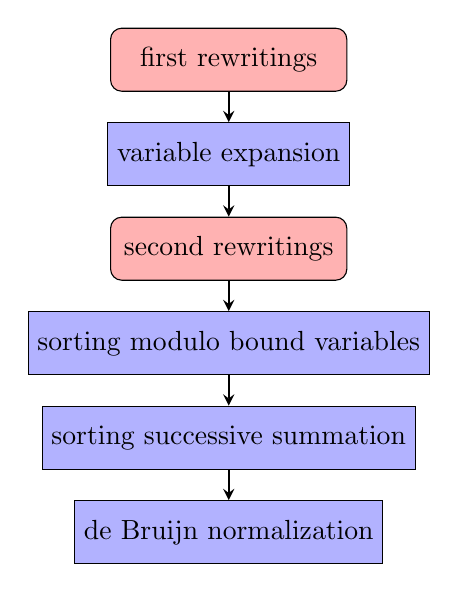
\begin{tikzpicture}[node distance=1.2cm]

    % \node (rename) [process] {rename unique bound variable names};
    \node (rewrite1) [rewriting] {first rewritings};
    \node (expansion) [process, below of=rewrite1] {variable expansion};
    \node (rewrite2) [rewriting, below of=expansion] {second rewritings};
    \node (sorting) [process, below of=rewrite2] {sorting modulo bound variables};
    \node (successive) [process, below of=sorting] {sorting successive summation};
    \node (deBruijn) [process, below of=successive] {de Bruijn normalization};

    % \draw [arrow] (rename) -- (rewrite1);
    \draw [arrow] (rewrite1) -- (expansion);
    \draw [arrow] (expansion) -- (rewrite2);
    \draw [arrow] (rewrite2) -- (sorting);
    \draw [arrow] (sorting) -- (successive);
    \draw [arrow] (successive) -- (deBruijn);

    \end{tikzpicture}
    \caption{A flowchart for normalization of Dirac notations.}
    \label{fig: normalization}
\end{figure}